\documentclass[11pt]{article}


%%%%%%%%%%%%%%%
\def\Type{ApplicationDJ}
\def\TypeNum{During-class for Application Day: Gradient Descent Method}
\def\TypeTitle{Gradient Descent}
\def\Semester{Fall 2025}
\def\Course{Math 1190/1210}
%\def\Targets{{\bf\color{Goldenrod}AD1}}
\def\desmosClassCode{{\bf ZAJ$3$AZ}}
\usepackage{preambleDJ}
\usepackage{graphicx}
\usepackage{footnote}
\usepackage{tikz}
\usepackage{pgfplots}
\usepackage[colorlinks=true, linkcolor=blue, urlcolor=blue]{hyperref}
%\pgfplotsset{compat=1.18}  % adjust to your version
\makesavenoteenv{minipage}
\begin{document}
%!TEX TS-program = xelatex
%!TEX encoding = UTF-8 Unicode



\pagestyle{otherpages}
\thispagestyle{firstpage}
\vspace*{.65in}


%!TEX TS-program = xelatex
%!TEX encoding = UTF-8 Unicode



%If Ada Lovelace\footnote{\url{https://en.wikipedia.org/wiki/Ada_Lovelace}} is the ``mother of programming" then 
{\bf Introduction}\\

\noindent
\begin{minipage}[c]{0.35\textwidth}
    \centering
    
\includegraphics[width=\linewidth]{Spring 2026/ApplicationDays/GradientDescent/images/feiFeiLiWiredCropped.png}
\end{minipage}
\hspace{0.02\textwidth}
\begin{minipage}[c]{0.63\textwidth}
Fei-Fei Li is known as the ``godmother of A.I'' for her groundbreaking contributions in computer vision and deep learning and as the creator of ImageNet\footnote{
See ``Godmother of A.I." Fei-Fei Li on technology development: ``The power lies within people" at \url{https://www.cbsnews.com/news/godmother-of-a-i-on-technology-development-fei-fei-li/}\\
or Britannica at \url{https://www.britannica.com/biography/Fei-Fei-Li}, The Guardian \href{https://www.theguardian.com/technology/2023/nov/05/ai-pioneer-fei-fei-li-im-more-concerned-about-the-risks-that-are-here-and-now}{\underline{here}} or \url{https://en.wikipedia.org/wiki/Fei-Fei_Li}
}.

\vspace{1em}

In this application, we will be exploring how the Gradient Descent method can be used for a supervised machine learning model that we have already seen in the Keeling Curve application. But before we do that, we need to refresh our memories about some properties of derivatives.

\medskip
{\bf Example 1: Function and Derivative}\\

Consider the function
\[
f(x) = x^2
\]

\begin{enumerate}
\item Compute the derivative:
\[
f'(x) = \rule{5cm}{0.4pt}
%\unline{1}{\blue{2x}}{.25}
\]

\item Evaluate at $x=3$:
\[
f'(3) = \rule{5cm}{0.4pt}
%\unline{1}{\blue{6}}{.25}
\]

\item Interpretation: since $f'(3) > 0$, the slope is positive. To decrease the value of $f(x)$ to be smaller than $f(3) = 9$, we should move to the left (decrease $x$) to go toward a smaller number. 
\end{enumerate}
\medskip
% Graph of f(x) = x^2 and tangent at x=3 with grid
\begin{center}
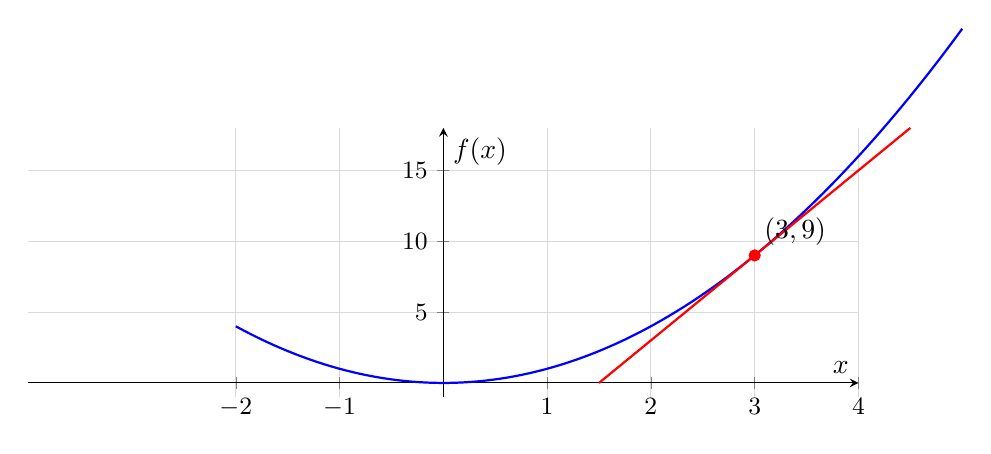
\begin{tikzpicture}
\begin{axis}[
    width=\linewidth,       % use full width of the minipage
    height=5cm,             % adjust height as needed
    axis lines=middle,
    xlabel=$x$, ylabel=$f(x)$,
    xmin=-4, xmax=4,
    ymin=-1, ymax=18,
    xtick={-2,-1,0,1,2,3,4},
    ytick={0,5,10,15,20},
    grid=both,              % add grid lines
    grid style={gray!30},   % light gray grid
    tick label style={font=\small}, % smaller labels
    enlargelimits=false,
    clip=false
]

% f(x) = x^2
\addplot [domain=-2:5, samples=100, blue, thick] {x^2};

% Tangent at x=3: f'(3) = 6
\addplot [domain=1.5:4.5, red, thick] {6*(x-3)+9};

% Mark the point (3,9)
\addplot[only marks, mark=*, red] coordinates {(3,9)};
\node[above right] at (axis cs:3,9) {$(3,9)$};

\end{axis}
\end{tikzpicture}
\end{center}
\end{minipage}
\newpage


















%%%%%%%%%%%%%%%%%%%%%%%%%%%%%%%%%%%%%%%%%%%%%%%%%%%%%%%%%%%%%%%%%%%%%%%%%%%%%%%%%%%%%%%%%%%%%%%%%%%%%%%%%%%%%%%%%%%%%%%%%%%%%%%%%%%%%%%%%%%%%%%%%%%%%%%%%%%%%%%%%%%%%%%%%%%%%%%%%%%%%%%%%%%%%%%%%%%%%%%%%%%%%%%%%%%%%%%%%%%%
\newpage
\section*{Introduction}

In this activity, we will use gradient descent to solve some real world calculus problems.
\section*{Application: Using Gradient Descent to Find an Unknown Constant}

\textbf{Motivation:} \\
Suppose water is flowing into a tank at a known rate $f(x)$ (gallons per minute). Then the total amount of water in the tank at time $t$ is given by an equation of the form:
\[
y'(t) = f(t)
\]
where the function $y(x)$ is telling us the  total amount of water flowing into the tank at time $t$. Using what we know about anti-derivatives and the Fundamental Theorem of Calculus, we know how to solve such an equation:

\begin{align*}
y'(t) &= f(t) \ \text{ so}\\
\int y'(t) \ dt  &= \int f(t) \ dt + C \  \text{ and }\\
y(t) &= \int f(t) \ dt + C
\end{align*}

where $C$ represents the \textbf{initial amount of water} in the tank.

\vspace{0.5cm}

\textbf{The Initial Problem:} \\
We do not know the value of $C$, but we are given a single  measurement:
\[
y(a) = y_a
\]
Our goal is to find the value of $C$ that makes our model match this data point. Thus telling us the initial amount of water in the tank.

\vspace{0.5cm}
\begin{enumerate}
\item \textbf{Define Our Model} \\
Let $G(t) = \int f(t) \ dt$ be any antiderivative of $f(t)$. Then our model is:
\[
\hat{y}(t) = G(t) + C
\]
This is our \textbf{prediction} for the amount of water.

\vspace{0.5cm}

\item \textbf{Measure the Error} \\
We want our model to match the known value at $x=a$. So we define the error:
\[
E(C) = \big(G(a) + C - y_a\big)^2
\]
This tells us how far off our prediction is.

\vspace{0.5cm}

\item \textbf{Adjust $C$ Using Gradient Descent} \\
To reduce the error, we compute the derivative:
\[
\frac{dE}{dC} = 2\big(G(a) + C - y_a\big)
\]

We can then update $C$ using:
\[
C_{\text{new}} = C_{\text{old}} - \alpha \cdot 2\big(G(a) + C_{\text{old}} - y_a\big)
\]
where $\alpha > 0$ is the \textbf{step size} (learning rate).
\end{enumerate}
\vspace{0.5cm}
%%%%%%%%%%%%%%%%%%%%%%%%%%%%%%%%%%%%%%%%%%%%%%%%%%%%%%%%%%%%%%%%%%%%%%%%%%%%%%%%%%%%%%%%%%%%%%%%%%%%%%%%%%%%%%%%%%%%%%%%%%%%%%%%%%%%%%%%%%%%%%%%%%%%%%%%%%%%%%%%%%%%%%%%%%%%%%%%%%%%%%%%%%%%%%%%%%%%%%%%%%%%%%%%%%%%%%%%%%%%%%%%%%%%%%%%%%%%%%%%%%%%%%%%%%%%%%%%%%%%%%%%%%%%%%%%%%%%%%%%%%%%

\section*{Example: Linear Activation}

Let's try the algorithm with a simple equation like:
\[
y'(t) = 2t
\]
\begin{enumerate}

\item  \textbf{Data}
Suppose we also know that $y(0) = 1$



\item \textbf{Initial guess}
Let:
\[
w_1 = w_2 = w_3 = 0, \quad b = 0
\]\\

Then:
\bigskip

$\hat{y_1}$ = \rule{5cm}{0.4pt}
\vspace{3cm}

%0\cdot 1 + 0\\
%&= 0\\
$\hat{y_2}$ = \rule{5cm}{0.4pt}
\vspace{3cm}

%0\cdot 2 + 0\\
%&=0
\bigskip

\item \textbf{Error}

$(y_1 - \hat{y_1})^2$= \rule{5cm}{0.4pt}
\vspace{3cm}

%(2 - 0)^2 \\
%= 4\\
$(y_2 - \hat{y_2})^2$ = \rule{5cm}{0.4pt}
\vspace{3cm}

%(4 - 0)^2\\
%= 16

$E(w,b)$ =  \rule{5cm}{0.4pt}
\vspace{3cm}

%= \frac{1}{2} (4 +  16) = 10


\item \textbf{Compute Partial Derivatives}

We compute:

\begin{align*}
\frac{\partial E}{\partial w} &= -\frac{2}{n} \sum_{i = 1}^2 (y_i - \hat{y}_i) t_i\\
&= -\frac{2}{2}\left((y_1 - \hat{y}_1) t_1 + (y_1 - \hat{y}_2) t_2\right)\\
\end{align*}
(Remember $f(t) = t$  \ So, $f(t_i) = t_i$ and $f'(t) = 1$)
\bigskip

For $i=1$:
\vspace{3cm}

$(y_1 - \hat{y}_1) t_1$ =  \rule{5cm}{0.4pt}
\vspace{3cm} 

%= (2 - 0)(1) \\
%= 2


For $i=2$:
\bigskip

$(y_2 - \hat{y}_2) t_2$  \rule{5cm}{0.4pt}
\vspace{3cm}
%= (4 - 0)(2) \\
%= 8


$\frac{\partial E}{\partial w_1}$ =  \rule{5cm}{0.4pt}
\vspace{3cm}

%-\frac{2}{2}(2 + 8) = -10
%\newpage
% Now partial derivative with respect to b
\begin{align*}
\frac{\partial E}{\partial b} &= -\frac{2}{n} \sum_{i=1}^2 (y_i - \hat{y}_i)\\
&= -\frac{2}{2} \left((y_1 - \hat{y}_1) + (y_2 - \hat{y}_2)\right)\\
\end{align*}

For $i=1$:
\[
y_1 - \hat{y}_1 = \rule{5cm}{0.4pt}
\]
\vspace{1.5cm}
% Example answer: 2 - 0 = 2

For $i=2$:
\[
y_2 - \hat{y}_2 = \rule{5cm}{0.4pt}
\]
\vspace{1.5cm}
% Example answer: 4 - 0 = 4

\[
\frac{\partial E}{\partial b} = \rule{5cm}{0.4pt}
\]
\vspace{1.5cm}
% Example answer: -(2 + 4) = -6

\item Update with gradient descent

Let's take $\alpha = 0.1$:
\bigskip

$w_{new}$ = \rule{5cm}{0.4pt}
\vspace{2cm}

%0 - 0.1(-10) = 1
$b_{new}$ = \rule{5cm}{0.4pt}
\vspace{2cm}

%
\end{enumerate}
%\newpage

\begin{enumerate}
    \item Compute one more update for $w$ and $b$.
    \vspace{4cm}
    
    \item Compute the new predictions.
    \vspace{4cm}
    
    \item Has the error decreased?
    \vspace{4cm}
    
\end{enumerate}
\newpage








\end{document}










































a \textbf{single-layer neural network} with one neuron to approximate the motion of a spring. Recall from physics that the position of a mass on a spring can often be modeled by a function of time, $y(t)$, for example:

\[
y(t) = A \sin(\omega t + \phi) + \text{noise}
\]

where $A$ is the amplitude, $\omega$ is the angular frequency, and $\phi$ is a phase shift. We will generate data from this type of motion and try to find a simple function that best fits it using a neural network trained with \textbf{gradient descent}.
\vspace{2cm}

\begin{figure}[h]
    
\includegraphics[width=0.7\linewidth]{Spring 2026/ApplicationDays/GradientDescent/images/SpringSystem.png}
    \caption{Spring system showing position $x$ and force $F$}
\end{figure}
\bigskip

\section*{Single-Layer Neural Network}

\textbf{Definition:} A \emph{single-layer neural network} (or a single neuron) takes in several input numbers and produces an output by combining them in a simple way.

Suppose we are given data points:
\[
(t_1, y_1), (t_2, y_2), \ldots, (t_n, y_n)
\]

In the simplest case, each input is just a single number. The neural network makes a prediction using:
\[
\hat{y_i}(t_i) = f(wt_i + b)
\]

where:
\begin{itemize}
    \item $w$ is a single \textbf{weight} (it controls how much $x$ matters)
    \item $b$ is a single \textbf{bias} (it shifts the output up or down)
    \item $f$ is an optional function (called an \textbf{activation function})
    \item $\hat{y_i}$ is the prediction for the ith y-value $y_i$
\end{itemize}

\textbf{Goal:} Find $w$ and $b$ so that $\hat{y}$ is as close as possible to the actual value $y$ for all data points.
\vspace{2cm}

We can see an illustration of a single layer single neuron neural network below:
\begin{center}
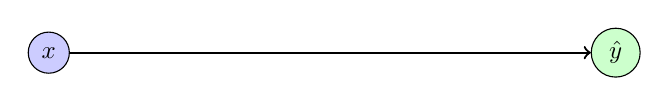
\begin{tikzpicture}[scale=1.2, every node/.style={scale=0.9}]
    % Input
    \node[circle, draw, fill=blue!20] (t) at (0,0) {$x$};
    % Neuron
    %\node[rectangle, draw, fill=yellow!30] (n) at (3,0) {Neuron $f(wx+b)$};
    % Output
    \node[circle, draw, fill=green!20] (y) at (6,0) {$\hat{y}$};
    % Arrows
    \draw[->, thick] (t) -- (y);
    %\draw[->, thick] (n) -- (y);
\end{tikzpicture}
\end{center}
\vspace{4cm}
%%%%%%%%%%%%%%%%%%%%%%%%%%%%%%%%%%%%%%%%%%%%%%%%%%%%%%%%%%%%%%%%%%%%%%%%%%%%%%%%%%%%%%%%%%%%%%%%%%%%%%%%%%%%%%%%%%%%%%%%%%%%%%%%%%%%%%%%%%%%%%%%%%%%%%%%%%%%%%%%%%%%%%%%%%%%%%%%%%%%%%%%%%%%%%%%%%%%%%%%%%%%%%%%%%%%%%%%%%%%

\textbf{Geometric Interpretation:} \\
The graph of $\hat{y}(x) = G(x) + C$ is just the graph of $G(x)$ shifted up or down.

\begin{itemize}
    \item If our prediction is too high at $x=a$, we decrease $C$.
    \item If our prediction is too low at $x=a$, we increase $C$.
\end{itemize}

So gradient descent is simply:
\begin{center}
\emph{``Slide the graph up or down until it passes through the point $(a, y_a)$.''}
\end{center}

\vspace{0.5cm}

\textbf{Connection to Neural Networks:} \\
This is an example of a very simple \textbf{neural network}:
\begin{itemize}
    \item Input: $x$
    \item Output: $\hat{y}(x) = G(x) + C$
    \item Parameter: $C$
\end{itemize}

Even though this model is simple, it uses the same ideas as larger neural networks:
\begin{itemize}
    \item Make a prediction
    \item Measure the error
    \item Adjust parameters to reduce the error
\end{itemize}

\vspace{0.5cm}

\textbf{Connection to the App:} \\
In the app, you will:
\begin{itemize}
    \item See the graph of $G(x)$
    \item Adjust $C$ using a slider (shifts the graph up/down)
    \item Observe the error value
    \item Run gradient descent to automatically find the correct $C$
\end{itemize}

\vspace{0.5cm}

\textbf{Key Idea:} \\
We already know the \emph{shape} of the solution from the integral. \\
Gradient descent helps us find the correct \emph{vertical position} of the graph.

\[
\boxed{\text{Gradient descent = adjusting } C \text{ until the graph matches reality}}
\]

%%%%%%%%%%%%%%%%%%%%%%%%%%%%%%%%%%%%%%%%%%%%%%%%%%%%%%%%%%%%%%%%%%%%%%%%%%%%%%%%%%%%%%%%%%%%%%%%%%%%%%%%%%%%%%%%%%%%%%%%%%%%%%%%%%%%%%%%%%%%%%%%%%%%%%%%%%%%%%%%%%%%%%%%%%%%%%%%%%%%%%%%%%%%%%%%%%%%%%%%%%%%%%%%%%%%%%%%%%%%
\newpage
Here's how the whole process would go:
\begin{enumerate}
    \item We start with a collection of data points $(t_1, y_1), (t_2, y_2), \ldots, (t_n, y_n)$ taken as samples from our spring data.\\
    \item Next,we choose some initial values for $w$ and $b$ (usually $w = b = 0$) to \textit{initialize} our neural network. We then pick an activation function $f(x)$ and consider the value of $\hat{y_i} = f(w_it_i +b)$ as a prediction for each of the $y$-values of our data points.\\
    \item Next, we calculate the error $E(w,b) = \frac{1}{n} \sum_{i=1}^n \big(y_i - \hat{y}(t_i)\big)^2$\\
    \item Now, find the partial derivatives of the error function $\frac{\partial E(w,b)}{\partial w}$ \quad $\frac{\partial E(w,b)}{\partial b}$
    \item Finally, using gradient descent, we use the $w$ and $b$ derivatives of the error function to find the optimal $w$ and $b$ that will minimize the error between our predictions and the $y$-values of our dataset.
\end{enumerate}
%%%%%%%%%%%%%%%%%%%%%%%%%%%%%%%%%%%%%%%%%%%%%%%%%%%%%%%%%%%%%%%%%%%%%%%%%%%%%%%%%%%%%%%%%%%%%%%%%%%%%%%%%%%%%%%%%%%%%%%%%%%%%%%%%%%%%%%%%%%%%%%%%%%%%%%%%%%%%%%%%%%%%%%%%%%%%%%%%%%%%%%%%%%%%%%%%%%%%%%%%%%%%%%%%%%%%%%%%%%%

%%%%%%%%%%%%%%%%%%%%%%%%%%%%%%%%%%%%%%%%%%%%%%%%%%%%%%%%%%%%%%%%%%%%%%%%%%%%%%%%%%%%%%%%%%%%%%%%%%%%%%%%%%%%%%%%%%%%%%%%%%%%%%%%%%%%%%%%%%%%%%%%%%%%%%%%%%%%%%%%%%%%%%%%%%%%%%%%%%%%%%%%%%%%%%%%%%%%%%%%%%%%%%%%%%%%%%%%%%%%



\section*{Approximating Spring Data with a Single-Layer Neural Network}

Now, suppose we have a spring system with sampled data points $(t_1, y_1), \dots, (t_n, y_n)$, where $t_i$ represents the time and $y_i$ represents the measured displacement.






We will test out three types of activation functions \textit{linear, logarithmic and exponential} and manipulate the learning rate and number of steps for our gradient descent algorithm to try to get the optimal weights and biases to find the best function to approximate our data. Go to this link \href{https://woodword0-gradientdescentapplication2.hf.space/}{Open the Gradient Descent App}




to answer the following questions.

\begin{enumerate}
\item First start with a linear function from the drop down menu and set the learning rate to $alpha = 0.1$. Run the gradient descent for 20 steps. Record the values for $w$ and $b$ below and test your parameters. What is the error?
\vspace{4cm}

\item Now keep $\alpha$ the same as before but change the number of steps to 50. How did increasing the number of steps affect the error?
\vspace{4cm}

\item Change the number of steps back to 20 and change $\alpha$ to 0.01. How did decreasing the learning rate affect the error?
\vspace{4cm}

\item Do you think this is giving you a good approximation of the data?
\vspace{4cm}


\item How could you improve this approximation?
\end{enumerate}
%\newpage

\begin{enumerate}
\item Now select the logarithmic activation function from the drop down menu and set the learning rate to $alpha = 0.1$. Run the gradient descent for 20 steps. Record the values for $w$ and $b$ below and test your parameters. What is the error?
\vspace{4cm}

\item Now keep $\alpha$ the same as before but change the number of steps to 50. How did increasing the number of steps affect the error?
\vspace{4cm}

\item Change the number of steps back to 20 and change $\alpha$ to 0.01. How did decreasing the learning rate affect the error?
\vspace{4cm}

\item Do you think this is giving you a good approximation of the data?
\vspace{4cm}


\item How could you improve this approximation?
\end{enumerate}
\newpage

\begin{enumerate}
\item Now select the exponential activation function from the drop down menu and set the learning rate to $alpha = 0.1$. Run the gradient descent for 20 steps. Record the values for $w$ and $b$ below and test your parameters. What is the error?
\vspace{4cm}

\item Now keep $\alpha$ the same as before but change the number of steps to 50. How did increasing the number of steps affect the error?
\vspace{4cm}

\item Change the number of steps back to 20 and change $\alpha$ to 0.01. How did decreasing the learning rate affect the error?
\vspace{4cm}

\item Do you think this is giving you a good approximation of the data?
\vspace{4cm}


\item How could you improve this approximation?
\end{enumerate}
\newpage

\begin{enumerate}
    \item Select one function and by manipulating the learning rate and number of steps do your best to find the $w$ and $b$ that gives the lowest possible error. 
    \vspace{4cm}
    
    \item Write an expression for your activation function using the $w$ and $b$ that you found.
  \vspace{4cm}
    
    \item What are the units of the domain and range of this function?
      \vspace{4cm}
    \end{enumerate}



\end{document}